%!TEX root = ../main.tex

\begin{align*}
    \frac{\partial J_N}{\partial a_i} &= \frac{2}{N} \sum_{t=1}^N (-\sin(\omega_it))(y_i(t) - a_i\sin(\omega_it)-b_i\cos(\omega_it)) = 0 \\
    \frac{\partial J_N}{\partial b_i} &= \frac{2}{N} \sum_{t=1}^N (-\cos(\omega_it))(y_i(t) - a_i\sin(\omega_it)-b_i\cos(\omega_it)) = 0
\end{align*}

This is a $2 \times 2$ linear system which can be written in matrix form

\[
    \begin{bmatrix}
        \sum_{t=1}^N \sin(\omega_it)^2 & \sum_{t=1}^N \sin(\omega_it)\cos(\omega_it) \\
        \sum_{t=1}^N \sin(\omega_it)\cos(\omega_it) & \sum_{t=1}^N \cos(\omega_it)^2
    \end{bmatrix}
    \begin{bmatrix}
        a_i \\ b_i
    \end{bmatrix} =
    \begin{bmatrix}
        \sum_{t=1}^N y_i(t)\sin(\omega_it) \\
        \sum_{t=1}^N y_i(t)\cos(\omega_it)
    \end{bmatrix}
\]

At this point we prefer to go back to a \emph{sin-only} form ($B_i$, $\phi_i$) of the estimated sinusoid $\hat{y}_i(t)$:
\[
    \hat{B}_i\sin(\omega_it + \phi_i) = \hat{B}_i\sin(\omega_it)\cos(\hat{\phi}_i) + \hat{B}_i\cos(\omega_it)\sin(\hat{\phi_i}) \stackrel{\text{!}}{=} \hat{a}_i\sin(\omega_it) + \hat{b}_i\cos(\omega_it)
\]

\[\Downarrow\]

\[
    \begin{cases}\label{sys:Bi}\tag{$\bigstar$}
         \hat{B}_i\cos(\hat{\phi}_i) = \hat{a}_i  \\
         \hat{B}_i\sin(\hat{\phi}_i) = \hat{b}_i 
    \end{cases}
\]

\[\Downarrow\]

\[
    \frac{\hat{b}_i}{\hat{a}_i} = \frac{\sin\hat{\phi}_i}{\cos{\hat{\phi}_i}} = \tan(\hat{\phi_i}) \qquad \hat{\phi}_i = \arctan \left( \frac{\hat{b}_i}{\hat{a}_i} \right)
\]
\[
    \hat{B}_i = \frac{\frac{\hat{a}_i}{\cos\hat{\phi}_i} + \frac{\hat{b}_i}{\sin\hat{\phi}_i}}{2} \quad \text{average of the the 2 equation in \eqref{sys:Bi}}
\]

Therefore, we have now found a bidirectional mapping $ \{ \hat{a}_i, \hat{b}_i \} \iff \{ \hat{B}_i, \hat{\phi}_i \}$.

Repeating the experiment and pre-processing for the $H$ experiments we can compute 

\begin{align*}
    \{ \hat{B}_1, \hat{\phi}_1 \} &\mapsto \frac{\hat{B}_1}{A_1} e^{j\hat{\phi}_1} \\
    \{ \hat{B}_2, \hat{\phi}_2 \} &\mapsto \frac{\hat{B}_2}{A_2} e^{j\hat{\phi}_2} \\
    \vdots& \\
    \{ \hat{B}_H, \hat{\phi}_H \} &\mapsto \frac{\hat{B}_H}{A_H} e^{j\hat{\phi}_H} \\
\end{align*}

where each $\frac{\hat{B}_i}{A_i} e^{j\hat{\phi}_i}$ is a complex number that is the estimated point at frequency $\omega_i$ of the frequency response of the transfer function $W(z)$ from the input $u(t)$ to the output $y(t)$ of the system.

\begin{recall}[Frequency Response Theorem for LTI systems]
    If for a LTI system characterized by \gls{tf} $W(z)$ the input is $A_i \sin (\omega_i t)$ and the output is $\hat{B}_i \sin (\omega_i t + \hat{\phi}_i)$, then $W(z=e^{j \omega_i}) = \frac{\hat{B}_i}{A_i} e^{j\hat{\phi}_i}$ is the corresponding frequency response of the system at that frequency ($\omega_i$).
    
    In particular, $\frac{\hat{B}_i}{A_i}$ is the ratio between the output and input amplitude and $\hat{\phi}_i$ is the phase shift.
\end{recall}

We can now plot these H point in a classical \emph{Bode plot} exploiting that $|W(e^{j \omega_i})| = \frac{\hat{B}_i}{A_i}$ and that $\angle W(e^{j \omega_i}) = \hat{\phi}_i$.

\begin{figure}[H]
    \centering
    \begin{tikzpicture}[node distance=1.5cm,auto,>=latex']
        \draw[->] (0,0) -- (5,0) node[right] {$\omega$};
        \draw[->] (0,-1.5) -- (0,3) node[left] {$|\cdot|$};
        \draw[domain=0:4,mark=*,only marks,samples=8,variable=\x] plot ({\x},{5*log10(2/(1+((2^\x)^2)/100))});
        \draw (4,0.1) -- ++(0,-0.2) node[below] {$\omega_H$};

        \draw[->] (0,-3) -- (5,-3) node[right] {$\omega$};
        \draw[->] (0,-4.5) -- (0,-1.7) node[left] {$\angle\cdot$};
        \draw[domain=0:4,mark=*,only marks,samples=8,variable=\x] plot ({\x},{2*(atan(2/(1+((2^\x)^2)/100))/180*3.14)-5.2});
        \draw (4,-2.9) -- ++(0,-0.2) node[below] {$\omega_H$};
    \end{tikzpicture}
\end{figure}

At the end of \emph{step 1} we have a frequency-domain dataset ($H$ values) representing $H$ estimated points of the frequency response of the system.

\paragraph{Step 2} Parametric model class (\gls{tf}) selection

\[
    \Mc(\theta): W(z; \theta) = \frac{b_0+b_1z^{-1}+\cdots+b_pz^{-p}}{1+a_1z^{-1}+\cdots+a_nz^{-n}}z^{-1}
    \qquad
    \theta = \begin{bmatrix}
        a_1 \\ \vdots \\ a_n \\ b_0 \\ \vdots \\ b_p
    \end{bmatrix}
\]

\begin{obs}[Model order selection]
    In this case the order is composed by 2 parameters $n$ and $p$:
    use cross-validation approach (or visual fitting in the Bode diagram) for finding the best choice of these parameters.
\end{obs}

\paragraph{Step 3} New performance index: variance of the error in frequency domain.

\[
    J_H(\theta) = \frac{1}{H} \sum_{i=1}^H \left | W(e^{j\omega_i}; \theta) - \frac{\hat{B}_i}{A_i}e^{j\hat{\phi}_i} \right | ^2
\]

where $W(e^{j\omega_i}; \theta)$ is the modeled frequency response and $\frac{\hat{B}_i}{A_i}e^{j\hat{\phi}_i}$ is the measured frequency response.

\paragraph{Step 4} Optimization

\[
    \hat{\theta}_H = \argmin_\theta J_H(\theta)
\]

Usually $J_H(\theta)$ is a \emph{non-quadratic} and \emph{non-convex function}; Thus, iterative optimization methods are needed.

\paragraph{Conclusion} We have obtained the estimated model which is a \gls{tf}

\[
    \Mc(\hat{\theta}_H): W(z; \hat{\theta}_H)
\]


\begin{remark}[Frequency bandwidth selection $\omega_H =\; ?$]
    Theoretically the standard best solution should be $H$ points distributed uniformly from 0 to $\omega_N$ (Nyquist freq.).

    In practice it's better to concentrate the experimental effort in a smaller and more focused bandwidth.

    \begin{figure}[H]
        \centering
        \begin{tikzpicture}[node distance=1.5cm,auto,>=latex']
            \draw[->] (0,0) -- (5,0) node[right] {$\omega$};
            \draw (0,0.1) -- (0,-0.1) node[below] {$0$};
            \draw (0.8,0.1) -- (0.8,-0.1) node[below] {$\omega_c$};
            \draw (2,0.1) -- (2,-0.1) node[below] {$\omega_N$};
            \draw (4,0.1) -- (4,-0.1) node[below] {$\omega_S$};
        \end{tikzpicture}
    \end{figure}

    where $\omega_c$ is the \emph{expected cut-off frequency} of the closed system.
    
    \textbf{Rule of thumb}: $\omega_H \approx 3\omega_c$

    \paragraph{Example} The Electronic Stability Control (ESC) system has an expected bandwidth of $\omega_c \approx 4 \text{Hz}$, so $\omega_H \approx 12\text{Hz}$.
\end{remark}

\begin{remark}[Emphasis on special frequency range]
    In some cases, between $\omega_1$ and $\omega_H$, we want to be more accurate in system identification in some frequency regions (typically around cut-off-frequency or around resonances).
    
    %TODO: replace this img with tikz figure
    \begin{figure}[H]
        \centering
        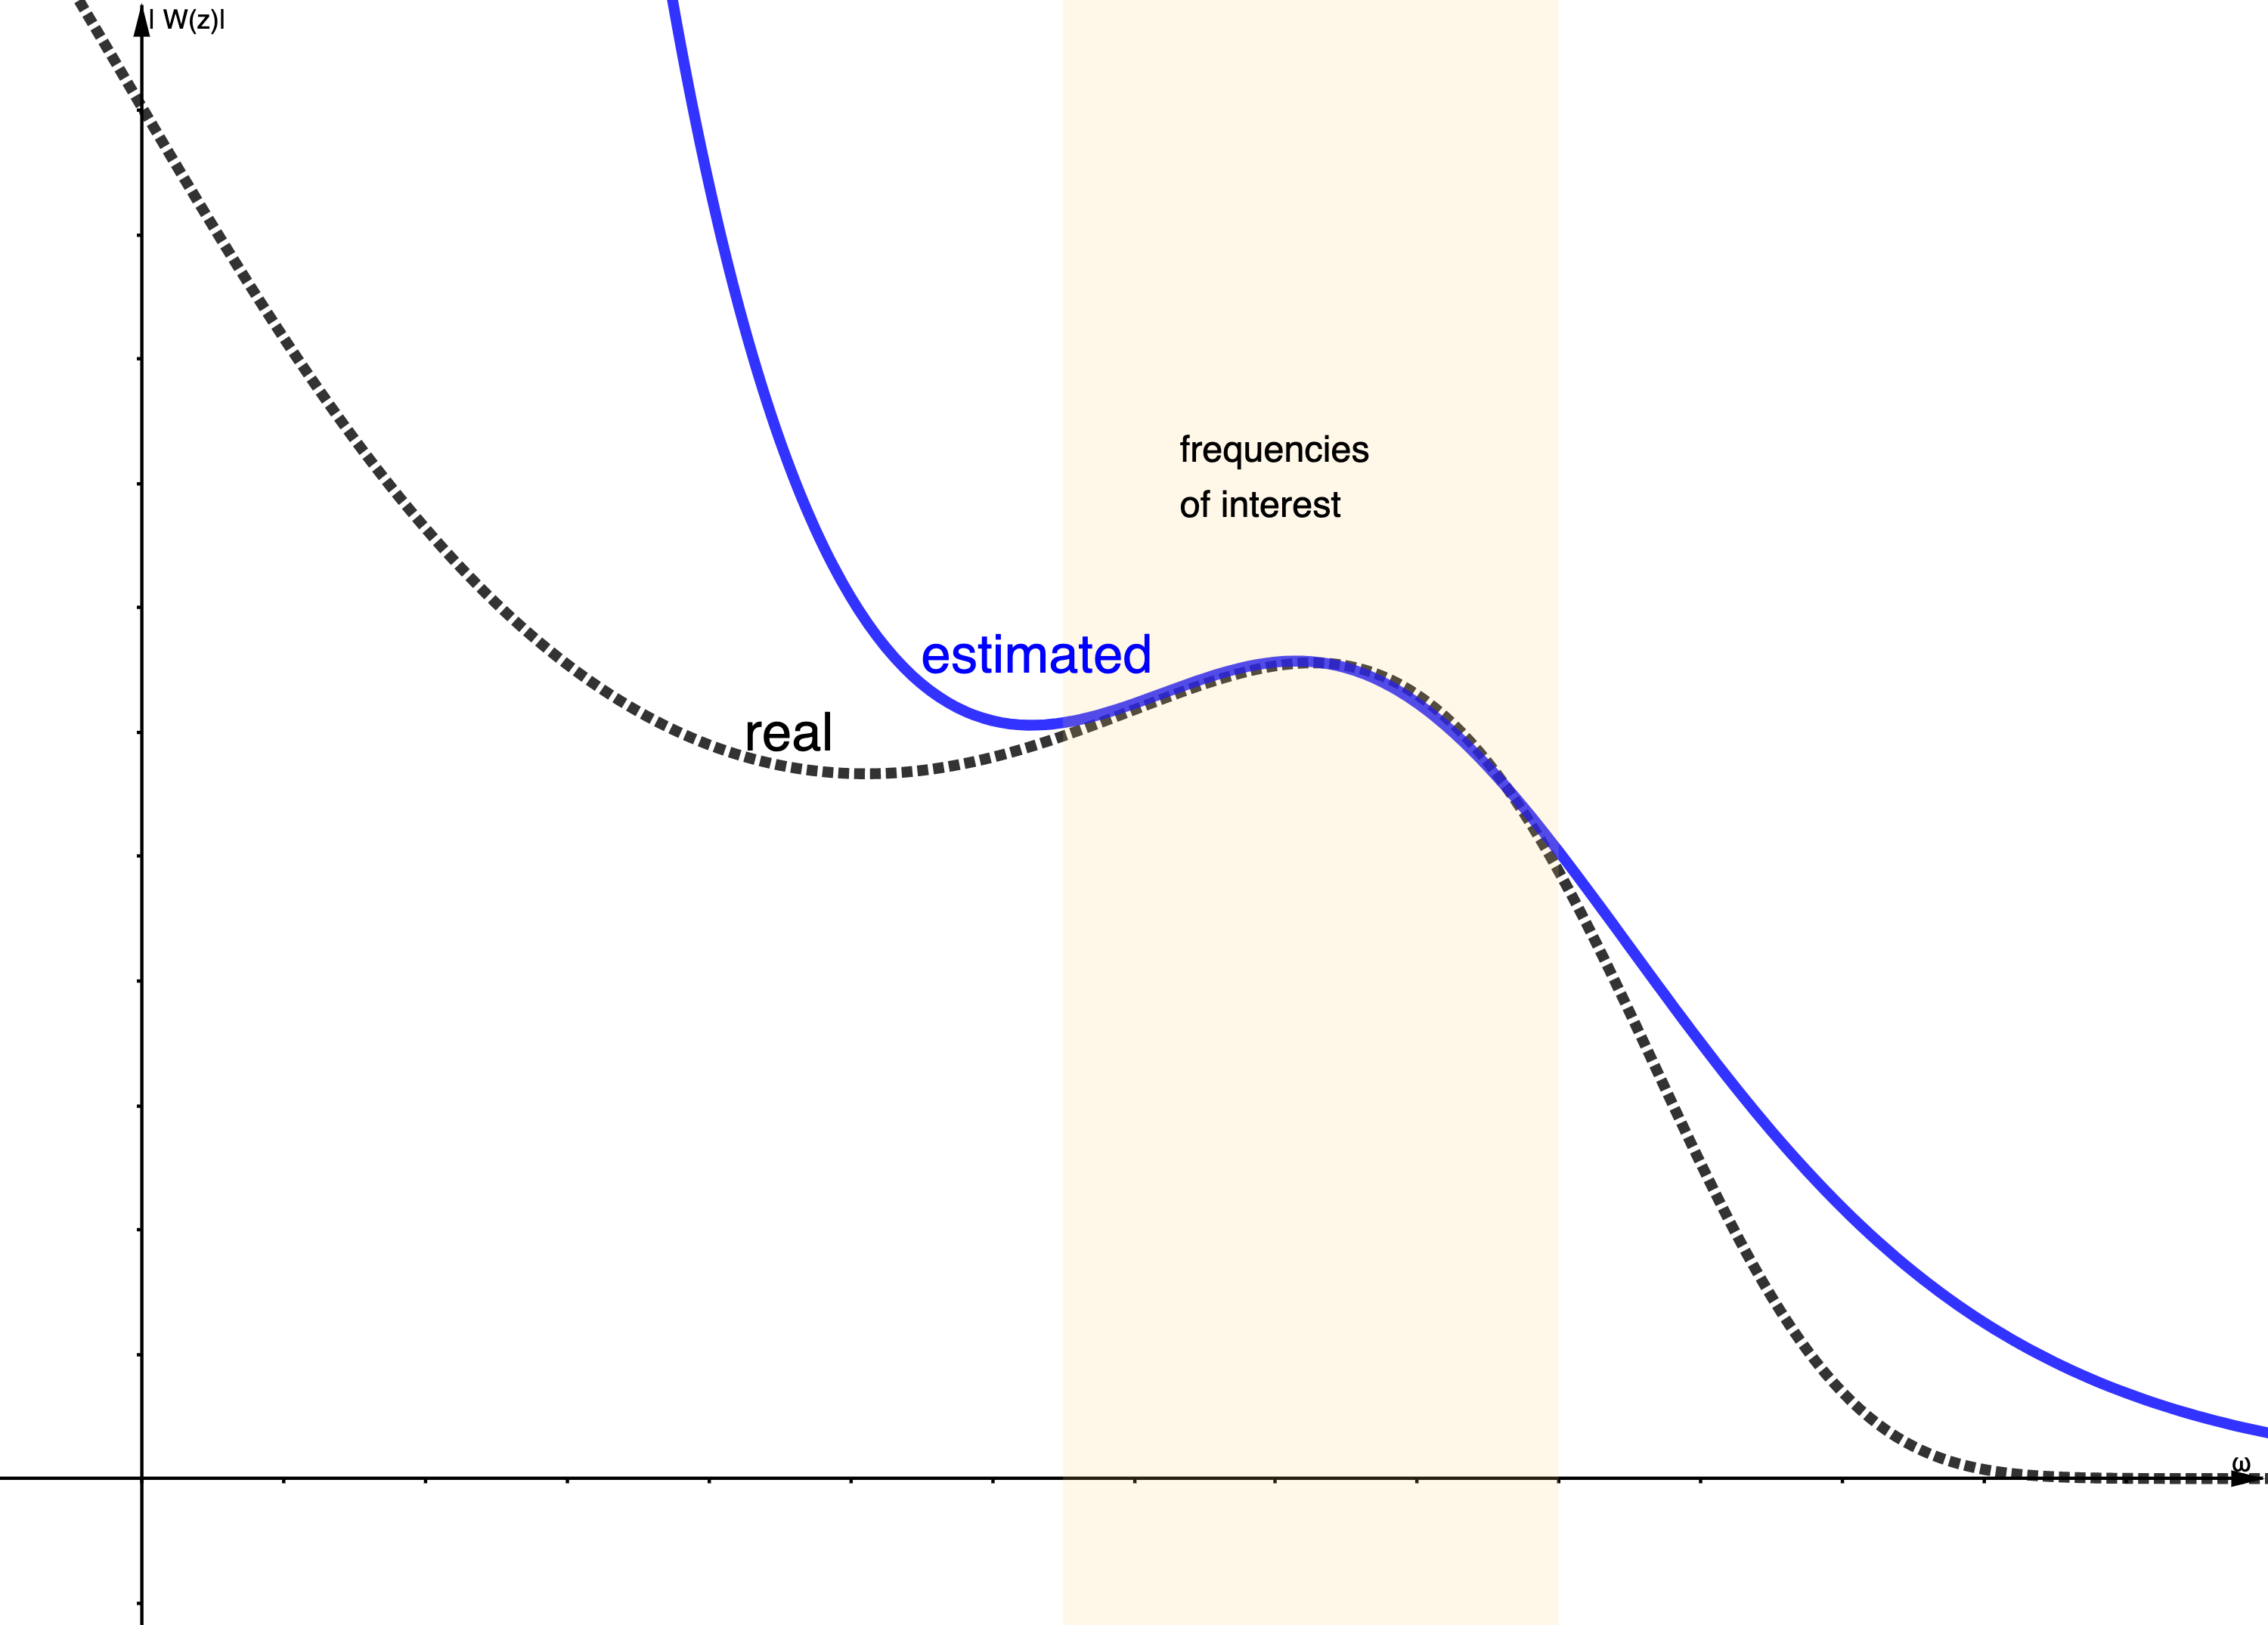
\includegraphics[scale=4.5]{./img/freq-emphasis.png}
    \end{figure}

    We can manage this selected focus on estimation precision using non-uniform weights $\lambda_i$ (different weights for different frequencies).

    \begin{figure}[H]
        \centering
        \begin{tikzpicture}[node distance=2.5cm,auto,>=latex']
            \begin{axis}[axis lines=none,ymax=2.5]
                \addplot[color=blue,mark=square]
                    coordinates {
                        (0,1)(1,1)(2,1)(3,1.2)(4,2)(5,1.2)(6,1)(7,1)(8,1)
                    };
            \end{axis}

            \draw[->] (-0.5,0) -- (7,0) node[right] {$\omega$};
            \draw[->] (0.5,-0.5) -- (0.5,5) node[left] {$\lambda_i$};
            \node at (0.1,0.5) {$1$};
            \draw (6.3,0.1) -- (6.3,-0.1) node [below] {$\omega_H$};
            \draw (1.3,0.1) -- (1.3,-0.1) node [below] {$\omega_1$};
            \draw (2,0.1) -- (2,-0.1) node [below] {$\omega_2$};
            \draw (3.5,0.1) -- ++(0,-0.2) node [below] {$\omega_x$};
        \end{tikzpicture}
    \end{figure}
    
    where $\omega_x$ is the frequency of interest.
    
    
    The performance index can be redefined:
    \[
        \tilde{J}_H (\theta) = \frac{1}{H} \sum_{i=1}^H \lambda_i \left(W(e^{j\omega_i};\theta) - \frac{\hat{B}_i}{A_i}e^{j\hat{\phi}_i}\right)^2
    \]

    Another \emph{trick}: more dense $\omega_i$ spacing in the frequency region of special interest (not really used).
\end{remark}

\begin{remark}[Single experiment]
    Sometimes the set of $H$ independent single-sinusoid experiments can be replaced by a long single ``sine-sweep'' experiment, that is to measure the frequency response of the system when the input is sinusoid that starts with frequency $\omega_1$ and amplitude $A_1$ and ends with frequency $\omega_H$ and amplitude $A_H$. 

    \begin{figure}[H]
        \centering
        \begin{tikzpicture}[node distance=2.5cm,auto,>=latex']
            \draw[->] (-0.5,0) -- (5,0) node[right] {$t$};
            \draw[->] (0,-1) -- (0,2) node[left] {$u(t)$};
            \draw[domain=0:4.5,samples=100,smooth,variable=\x,blue] plot ({\x},{cos(\x*180/3.14*(\x^1.7+5))*e^(-\x/2.5)});
        \end{tikzpicture}
        \caption*{Slowing-varying sinusoid with increasing frequency and decreasing amplitude.}
    \end{figure}

    The output will be a single long signal $y(t)$.
    
    We can cut a-posteriori the signal into $H$ pieces, and then back to the standard procedure
    or we can directly compute an estimation of $\hat{W}(e^{j\omega})$ as a ration of the output and input spectra %(recalling that $\Gamma_y(\omega) = |W(z)|^2 \Gamma_u(\omega)$)

    \[
        \hat{W}(e^{j\omega}) = \frac{\hat{\Gamma}_y(e^{j\omega})}{\hat{\Gamma}_u(e^{j\omega})}
    \]

    We can fit the estimated $\hat{W}(e^{j\omega})$ with the model frequency response $W(e^{j\omega}; \theta)$ in the performance index.
    
    \[
        \frac{1}{H} \sum_{i=1}^H \left| W(e^{j \omega_i}; \theta) - \hat{W}(e^{j \omega_i}) \right|^2
    \]
    where, similarly, $W(e^{j\omega_i}; \theta)$ is the modeled frequency response and $\hat{W}(e^{j \omega_i})$ is the measured frequency response.
    
    This experiment is quicker but has usually a lower signal-to-noise-ration.
\end{remark}

\begin{remark}[Experiment on unstable system]
    What happen if the system is \emph{open-loop} unstable? We have to stop the experiment because of the instability of the output (which of course diverges).
    
    \begin{figure}[H]
    \centering
    \begin{tikzpicture}[node distance=1.5cm,auto,>=latex']
        \node[block] (sys) {$\Sys$};
        \node[left of=sys, node distance=3cm] (in) {};
        \node[left of=in] (in2) {};
        \node[right of=sys, node distance=2.5cm] (out) {};
        \node[right of=out, node distance=2cm] (out2) {};

        \draw[xshift=-4cm,yshift=0.5cm,scale=0.2,domain=0:4*pi,smooth,variable=\x] plot ({\x},{sin(8*\x r)});

        \draw[xshift=1cm,yshift=0.5cm,scale=0.2,domain=0:4*pi,smooth,variable=\x,samples=100] plot ({\x},{sin(8*\x r + 10)*exp(0.15*\x)});
        \draw[->] (in2) -- (sys);
        \draw[->] (sys) -- (out2);
    \end{tikzpicture}
\end{figure}
    
    We can avoid this problem by performing the experiment in \emph{closed-loop}  and adding a \emph{stability controller}.
    
        \begin{figure}[H]
        \centering
        \begin{tikzpicture}[node distance=2.5cm,auto,>=latex']
            \node [block,align=center] (stab) {stability\\controller};
            \node [block] (sys) [right of=sum, node distance=2cm]{$\Sys$};
            \node [coordinate] (split) [right of=sys, node distance=1cm]{};
            \node [] (end) [right of=split, node distance=3cm]{$y(t)$};
            \node [] (in) [left of=stab, node distance =4cm]{$\bar{y}(t)$};
            \node [coordinate] (mid) [below of=sum, node distance=1.5cm] {};

            \draw[->] (in) -- (stab);
            \draw[->] (stab) -- (sys);
            \draw (sys) edge (split);
            \draw[->] (split) -- (end);
            \draw (split) |- (mid);
            \draw[->] (mid) -| (stab);
            
            \draw[xshift=-3.6cm, yshift=0.5cm, scale=0.2, domain=0:4*pi, smooth, variable=\x] plot ({\x}, {sin(8*\x r)});
            \draw[blue, xshift=1cm, yshift=0.5cm, scale=0.2, domain=0:4*pi, smooth, variable=\x] plot ({\x}, {1.5*sin(8*\x r + 5)});
            \draw[blue, xshift=4.5cm, yshift=0.5cm, scale=0.2, domain=0:4*pi, smooth, variable=\x] plot ({\x}, {0.7*sin(15*\x r + 7)});
            
        \end{tikzpicture}
    \end{figure}
    
    where the blue sinusoids are the signal reflecting the dynamic of the system and, measuring them, they will compose the dataset I/O of the system. 
    
    \textbf{Note} that the model identified using that dataset will be a model of an unstable system.
    
    This is just a trick to collect data from an unstable system.
\end{remark}



\section{Comparison between time domain and frequency domain parametric methods}

\paragraph{Frequency domains}
\begin{description}
    \item[Pro] Robust and very reliable because each experiment has a big signal-to-noise ratio (since we are forcing all the signal energy on a single clean sinusoid).
    \item[Pro] Intuitive since it is easy to understand.
    \item[Pro] Consistent with many control-design methods that work in the frequency domain.
    \item[Cons] More demanding in terms of design of the experiment.
    \item[Cons] Provides no noise model (unlike the \gls{pem} method of \gls{armax} system identification)
    \end{description}

\textbf{Note} that F.D. and T.D. methods should provide approximately the same result if done correctly.


\chapter{Software (virtual) Sensing model-based in feedback method using Kalman Filter framework}

In MIDA1 we have mostly used I/O \acrfull{tf} representations:
\[ y(t) = \frac{B(z)}{A(z)}u(t-k) + \frac{C(z)}{A(z)}e(t) \qquad e(t) \sim \WN \]


Kalman filter theory is fully based on \acrfull{ss} representation

\[
    \begin{cases}
        x(t+1) = Fx(t) + Gu(t) + v_1(t)  & \qquad v_1 \sim \WN \\
        y(t) = Hx(t) + \cancel{Du(t)} + v_2(t) & \qquad v_2 \sim \WN
    \end{cases}
\]

where we assume that the system model is given (typically obtained in a white-box approach): it's not a system identification problem! Indeed we are interested in the internal state of the system.

\begin{figure}[H]
    \centering
    \begin{tikzpicture}[node distance=2.5cm,auto,>=latex']
        \node [block, align=center] (sys) {$\Sys$ \\ \vspace{10pt} \qquad \\ \qquad$x(t)$};
        \node (in) [left of=sys, node distance=2cm] {$u(t)$};
        \node (out) [right of=sys, node distance=2cm]{$y(t)$};
        \node (wn1) [above of=sys, node distance=1.5cm, xshift=-1cm] {$v_1(t)$};
        \node (wn2) [above of=sys, node distance=1.5cm, xshift=1cm] {$v_2(t)$};

        \draw[->] (in) -- (sys);
        \draw[->] (sys) -- (out);
        \draw[->] (wn1) -- (sys);
        \draw[->] (wn2) -- (sys);
    \end{tikzpicture}
    \caption*{Two-noises model}
\end{figure}


\section{Motivation and Goals of Kalman Filter}

Given a model description $\{F, G, H\}$ and noises variances (not a system identification technique), with \acrfull{kf} theory we can address the following problems:

\begin{itemize}
    \item Find the $k$-steps ahead prediction of output: $\hat{y}(t+k|t)$ (already solved in MIDA1 with \gls{armax}).
    \item Find the $k$-steps ahead prediction of state: $\hat{x}(t+k|t)$.
    \item Find the filter of the state at present time: $\hat{x}(t|t)$. In practice it's a \emph{software-sensing} problem, which is the most important problem solved by Kalman filter (reason of why it is named Kalman \emph{filter}).
    \item Gray box system identification (see \nameref{ch5}). We have a recorded data-set and the model structure with some unknown parameters.
\end{itemize}


